\documentclass{ctexart}
\usepackage[utf8]{inputenc}
\usepackage{amsmath}
\usepackage{amsfonts}
\usepackage{amssymb}
\usepackage{makeidx}
\usepackage{graphicx}
\usepackage{CJK}
\usepackage{lipsum}
\usepackage{pdfpages}


%\begin{CJK}{UTF8}{gbsn}
\author{吴秉哲 1200010666}
\title{数值线性代数第二次上机作业}
\begin{document}
\maketitle
\section*{第二章习题}
\subsection*{习题1}
估计5到20阶Hilbert矩阵的$\infty$范数条件数:


本题使用了书中算法5.12(估计矩阵的1范数)。对于n阶的Hilbert
矩阵$H_n$,在估计$\lVert H^{-1}_{n} \lVert_{\infty}$的时候需要
求解方程$H^{T}_{n}\omega=x 和 H_nz=\upsilon,$我使用了
选列主元的Gauss消去法求解,得到了$\lVert H^{-1}_{n}
\lVert_{\infty}$的估计值。考虑到$H_n$的高度病态性,求解上面两个方程组可能会产生比较大的误差,故需要使用一种方法来检验。Matlab自带有矩阵
求逆函数inv()和求范数函数norm(),可以求出$H^{-1}_{n}$和
$\lVert H^{-1}_{n} \lVert_{\infty}$,经测试发现当n比较大的时候误差也很大的。但是目前没有
$H^{-1}_{n}$的精确值,无法判断该估计的误差大小,所以我就把用
书中算法估计的范数和用inv()函数求逆后再求的范数进行了比较。又
$\lVert H_{n} \lVert_{\infty}$的计算比较简单,误差应该相对较小,故我直接计算了$\kappa
_n=\lVert H^{-1}_{n} \lVert_{\infty}$$\lVert H_{n} \lVert_{\infty}$。计算结果如下表所示:
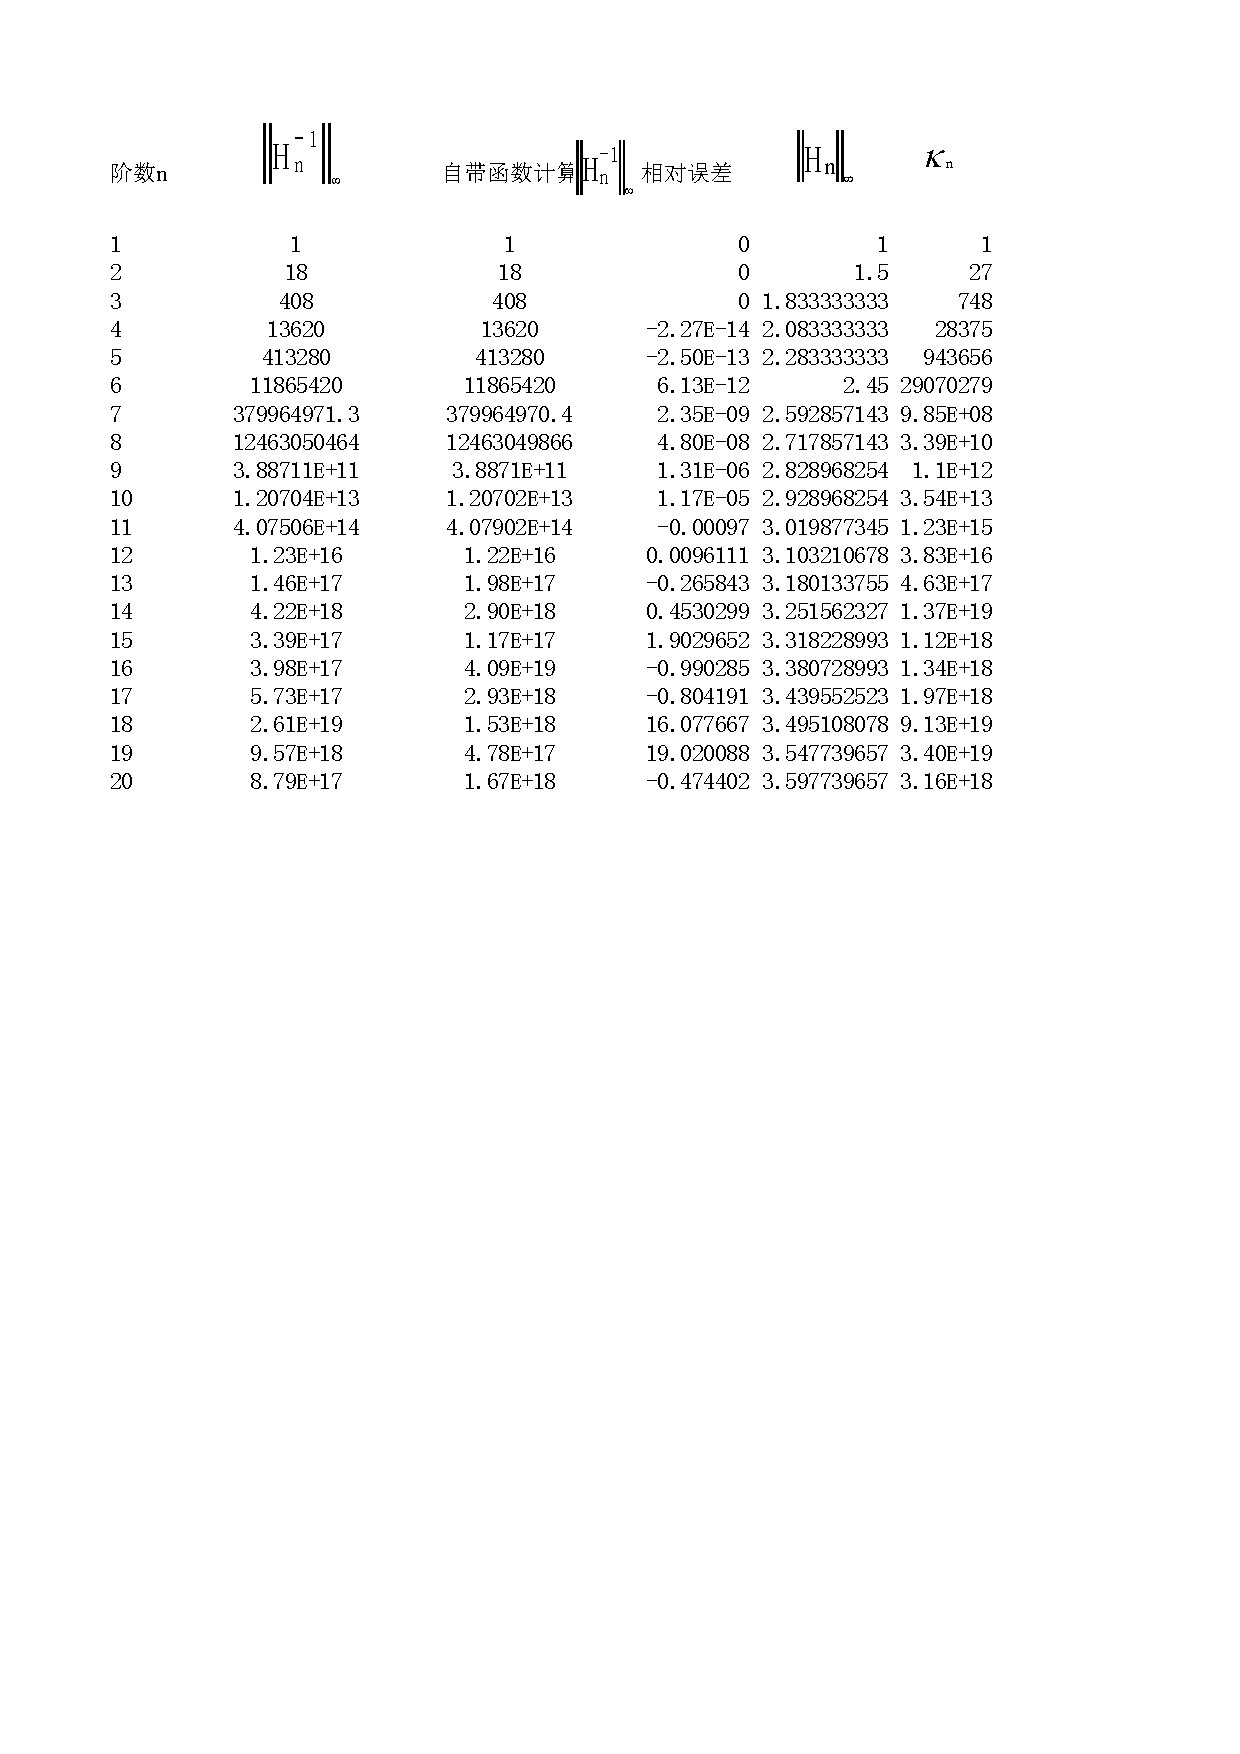
\includepdf{习题1.pdf}




从表中可以看出,
\begin{enumerate}
\item
$\lVert H^{-1}_{n} \lVert_{\infty}$随阶数的增长是近乎是
指数型的,但比指数慢,而$\lVert H^{-1}_{n} \lVert$基本是
一个常数,所以$\kappa_n 和\lVert H^{-1}_{n} \lVert_{\infty}$基本一样也是增长得很快,到13阶就已经达到了
$10^17$数量级,超出了机器精度。从维基百科上查到,$\kappa_n=
O(\dfrac{(1+\sqrt{2})^{4n}}{\sqrt{n}})$,符合计算结果
\item
而对$\lVert H^{-1}_{n} \lVert_{\infty}$的估计在n比较大的时候也明显产生了误差,无论是
算法5.12还是Matlab的自带函数,它们都不单调。我猜测$\lVert H^{-1}_{n} \lVert_{\infty}$应该随着n的增加单调上升,尚未查找到文献验证。
\item
Matlab的函数计算的结果和误差估计的相对误差随着n的增加而增加,整体也是比较小的,说明这种方法应该误差不大。在网上未查找到
$\lVert H^{-1}_{n} \lVert_{\infty}$的准确值来比较
\end{enumerate}
\subsection*{习题2}
估计解的误差与真实相对误差比较。
本题中x的分量服从$U(0,1)$分布,使用列主元Gauss消去法求解得到
$\widehat{\chi}$,并使用
$\dfrac{\kappa_{\infty}(A_n)\|r\|_{\infty}}{\|b\|_\infty}$来估计解的相对误差$\dfrac{\|x-\widehat{\chi}\|_\infty}{\|x\|_\infty}$.具体结果如下表:
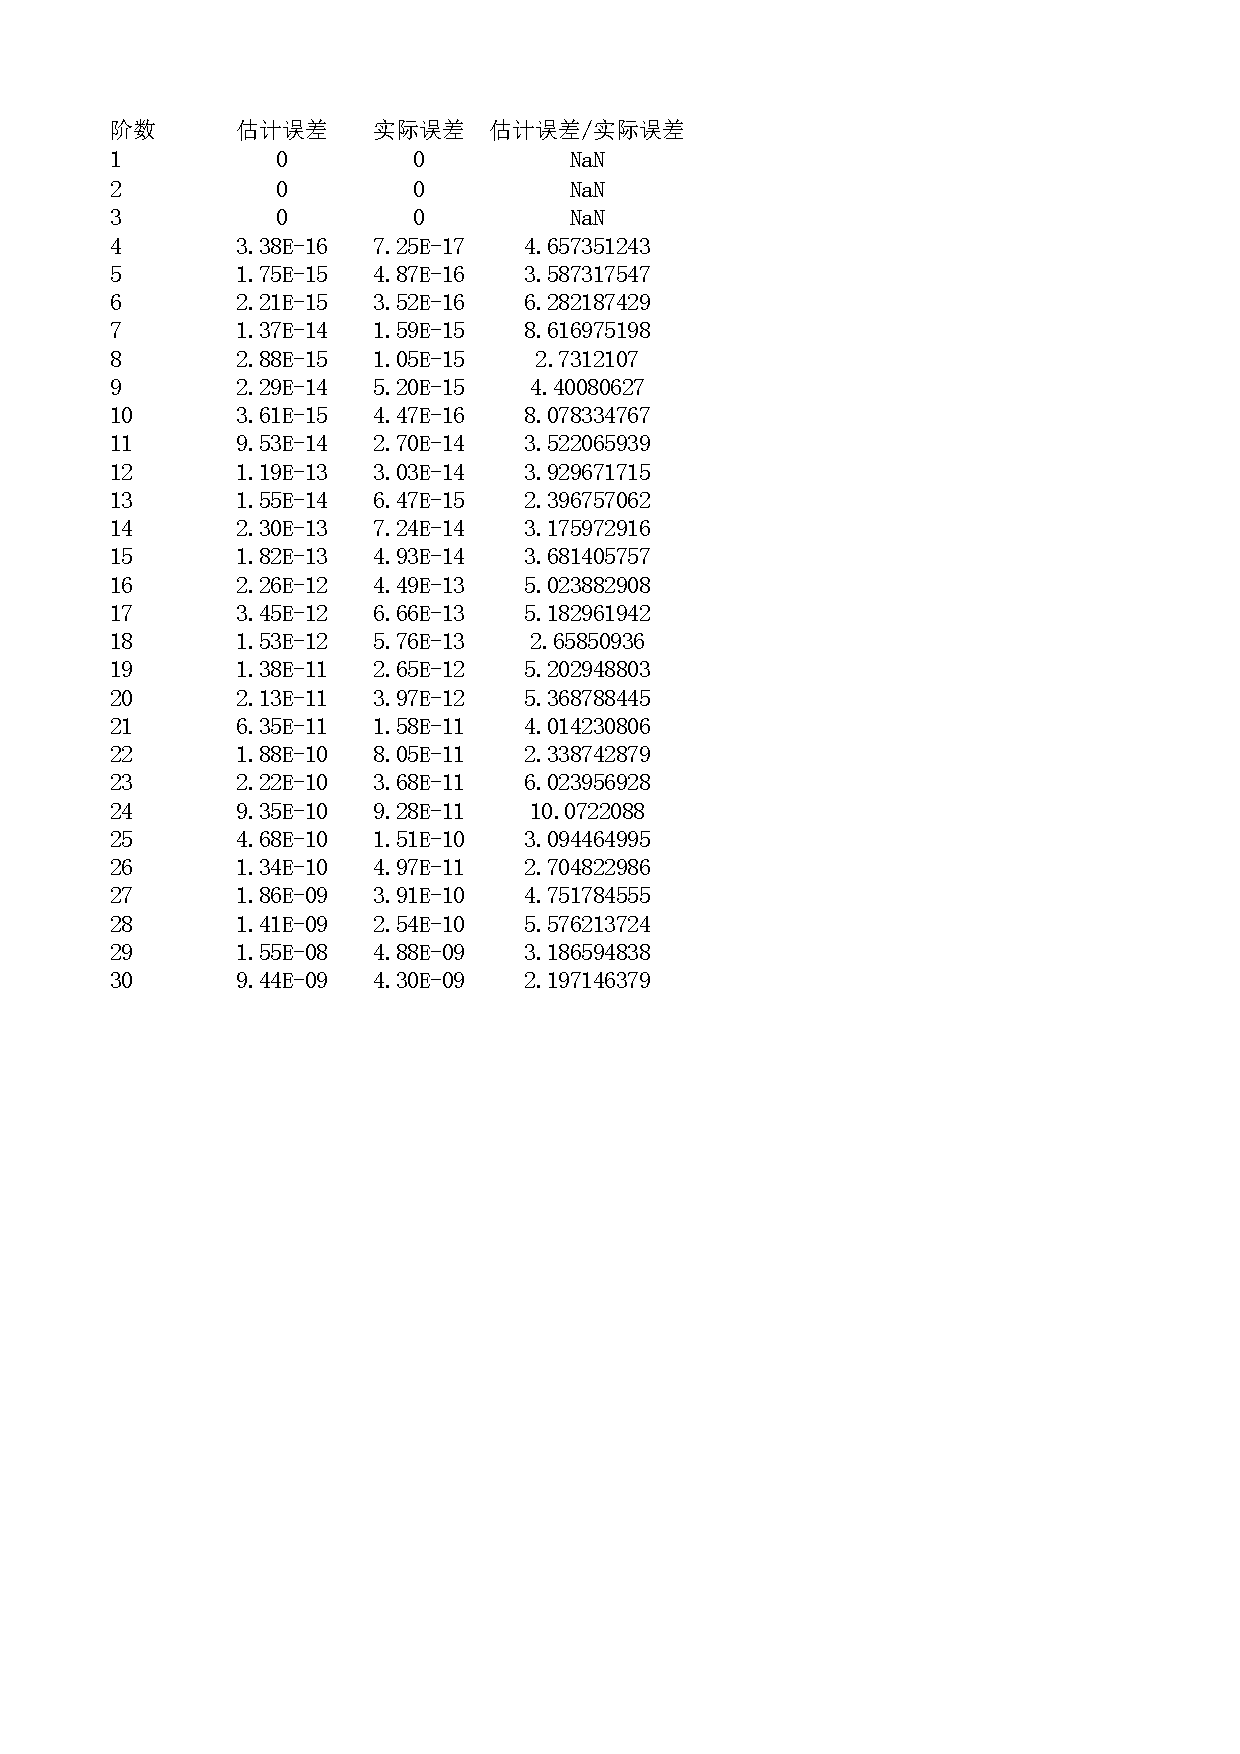
\includepdf{习题2.pdf}
从表中可见,
\begin{enumerate}
\item
估计的误差和实际的误差随阶数的增加而总体增加,并且总体来说误差非常小
\item
估计误差总是比实际误差大,而且理论推导证明这个估计误差应该大于
实际误差,这个结果说明得到的结果没有和理论推导矛盾
\item
估计误差是实际误差的10倍以内,大部分在5倍以内,并没有随着n的
增大而增大。说明这个估计是比较好的。
\end{enumerate}

\section*{第三章习题}
\subsection*{习题1}
用QR分解求解第一章的三个方程。

\begin{itemize}
\item 方程1

n=55;计算解的误差分量如下图:
\par
\centerline{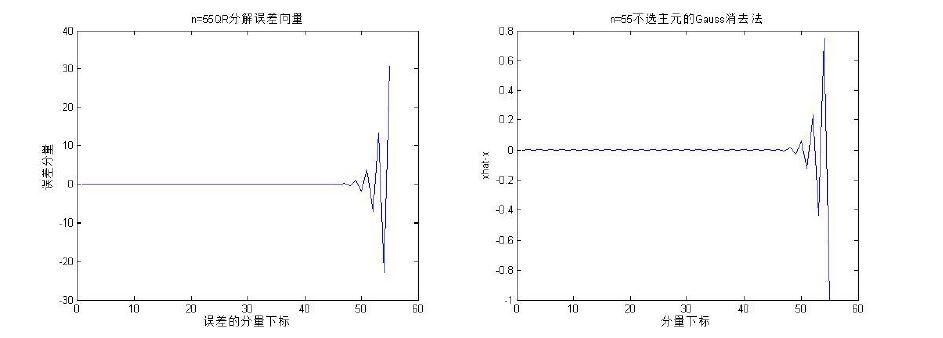
\includegraphics[height=5cm,width=15cm]{1.jpg}}
\par

\begin{enumerate}
\item
另人惊奇的是,使用Householder变换的QR分解最多只能解到
n=55的情况,阶数再大就会出现inf和NaN。查看运算中间结果
发现,$\|A(j:n,j)\|\rightarrow 0,$随着 $j\rightarrow
n$,导致解上三角方程时出现问题。
\item
查看中间结果还发现,$\beta \rightarrow 1,v\rightarrow
(1,-1,0,...,0)'$。
\item
和不选主元的Gauss消去法相比误差大约是其50倍,和选主元的更没法
比较了,有非常大的误差。但两者误差分量变换模式相似,都是前面的
分量误差小,之后越来越大,正负跳跃。
\end{enumerate}

\item 方程2

随机选择 结果如下图:
\par
\centerline{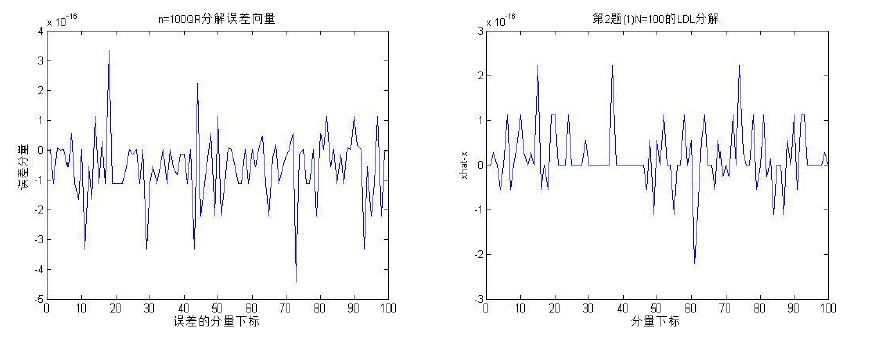
\includegraphics[height=5cm,width=15cm]{2.jpg}}
\par
\begin{enumerate}
\item
QR分解求解的误差很小,约为机器精度,和第一次作业中使用的
Gauss消去法,Cholesky分解和$LDL^T$表现相似。这是由于
矩阵A的良态
\item
解的误差分量变动很随机,没有明显规律,从大小来看应该也近似
服从正态分布。
\end{enumerate}
\item 方程3

Hilbert矩阵:

以下分别对n=14,40,100画出误差分量并与Cholesky,Gauss消去法
作比较:
\par
\centerline{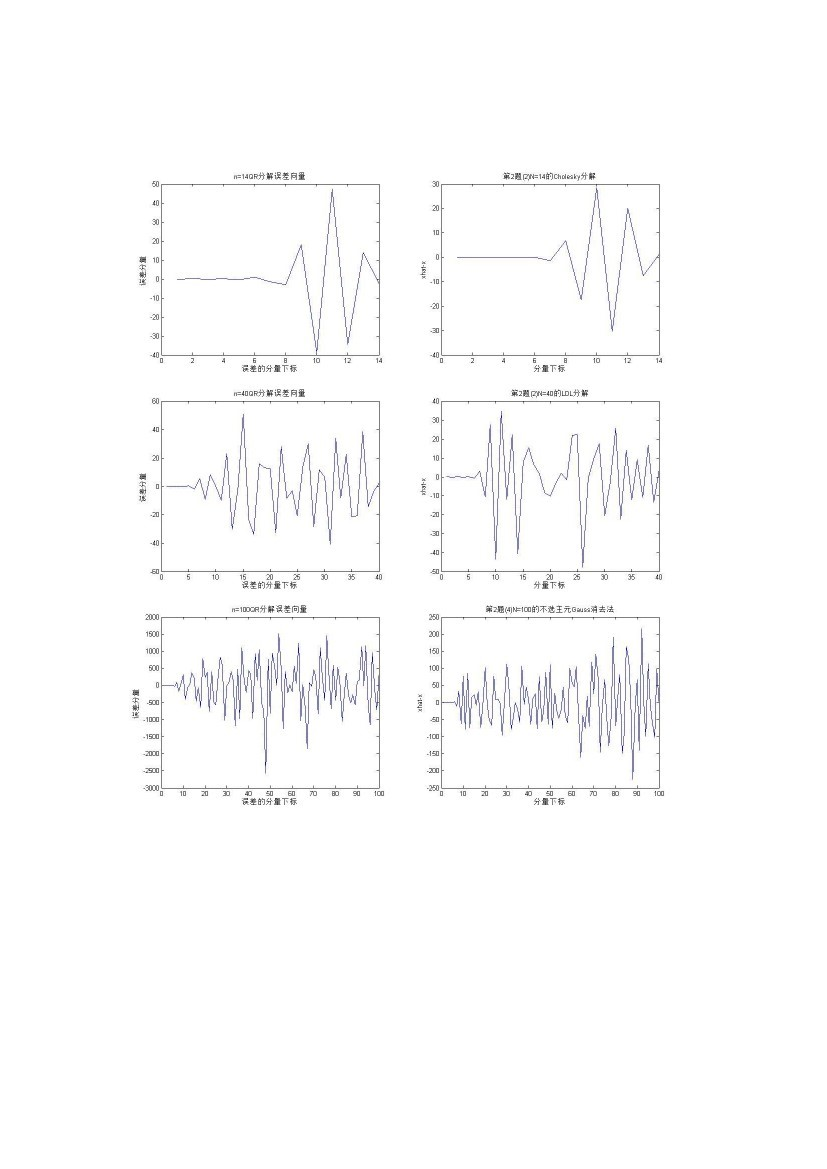
\includegraphics{3.jpg}}
\par
从以上图可以看到:
\begin{enumerate}
\item
QR分解可以对较大的n求解,比Choslesky强
\item
QR分解的误差也很大,n=14时,比Cholesky分解误差大,n=40
比$LDL^T$分解误差大,n=100是不选主元的Gauss分解误差的10倍
\item
无论哪种方法得到的误差模式都很相似,说明这是方程本身的特性,或者
说是矩阵的性质,和采取的计算方法无关。
\end{enumerate}
\end{itemize}
综上看来:
\begin{enumerate}
\item
虽然QR分解的运算量要更大,并且上课老师说这个方法要更精确,但是对
这三个方程并未表现出明显的差别。相反,QR方法的误差反而比第一章方法误差要大。
\item
这里的正交分解使用的是Householder变换,如果采用Givens变换
结果或许会有所差别。因为本次作业的时间限制,并未对其进行实验
\item
因为测试的方程组阶数都很小,没有发现明显的运算时间变化。
\item
观察发现对于同一方程组的不同方法计算得到的误差向量可能大小有很大差别,但是把向量归一化后,误差分量的变化模式都极为相像。
\end{enumerate}
\subsection*{第二题}
求解最小2乘问题,拟合抛物线

题目模型为$y=at^2+bt+c$,数据略,直接给出利用树上算法
得出的QR分解的结果:
\[y=1.0483t^2+0.9863t+0.9569\]
拟合抛物线与原始数据作图如下:
\par
\centerline{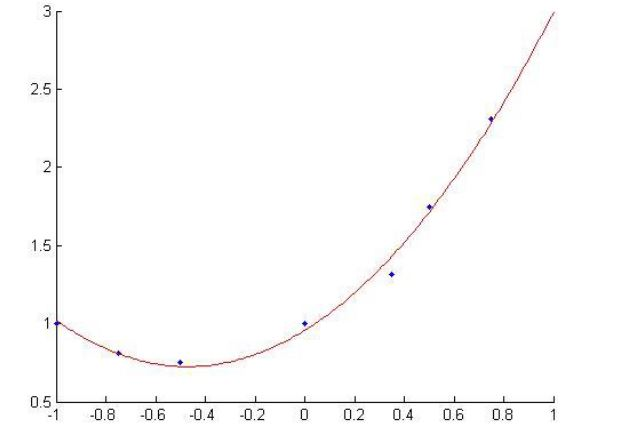
\includegraphics[height=5cm,width=10cm]{4.jpg}}
\par
从上图看出,拟合的效果还是不错的,说明方法是没错的
\subsection*{第三题}
求解多元回归的实际问题:

先给出书上算法得出的计算结果,在给出用专门的统计软件给出的结果。
对两个结果进行对比。
共有n=28个观测值,k=11个解释变量,直接给出QR分解求解此OLS
问题的解:
\par
\centerline{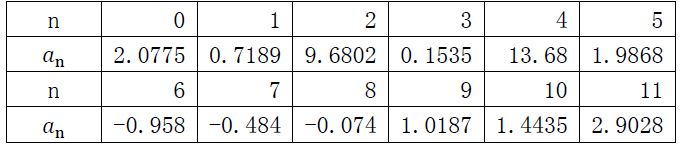
\includegraphics[height=4cm,width=20cm]{99.jpg}}
\par

其中$a_0$是截距项

另外使用stata对数据进行OLS回归可得如下结果:
\par
\centerline{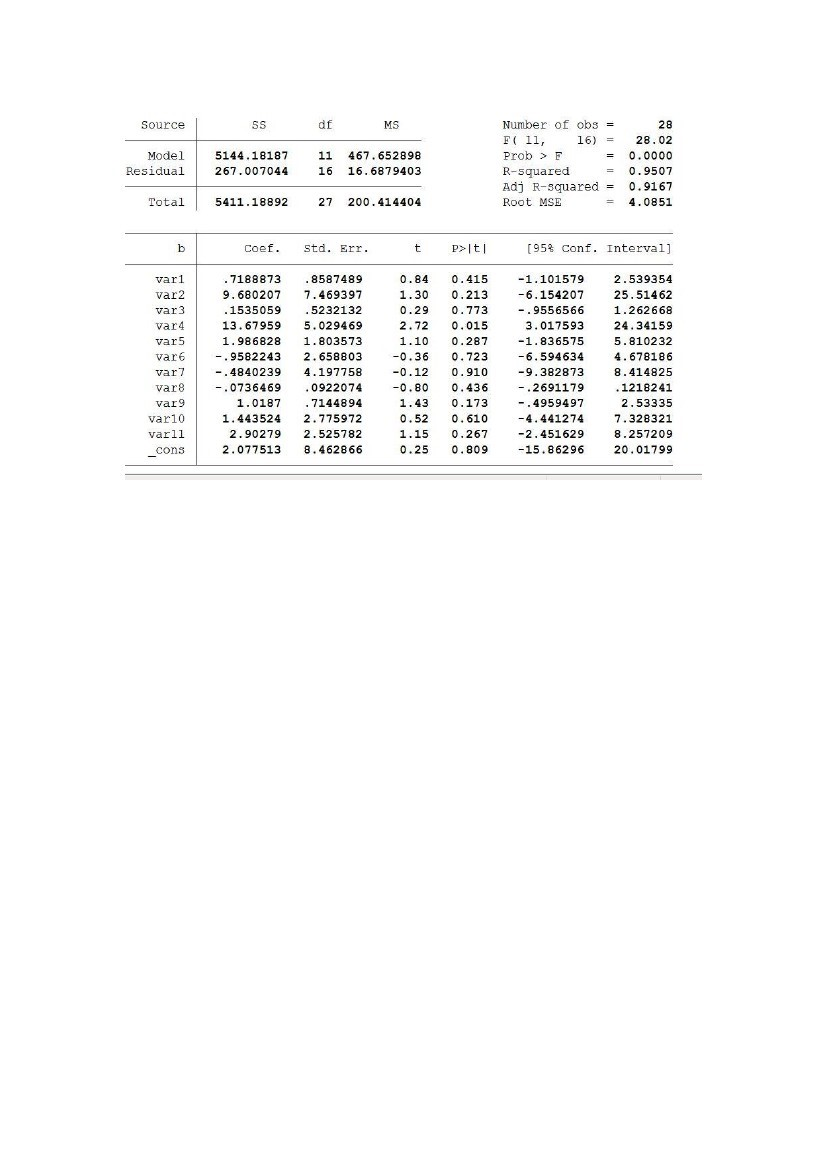
\includegraphics{5.jpg}}
\par
由上可以看出,两种方法对系数的估计是相同的。

从数据来看模型可能存在多重共线性的问题。

本次作业的代码全由Matlab编写,感觉比较简单,但是在估计矩阵
的无穷范数的问题上,以及用多种方法解方程,还是有很多地方很值的思考的。
%\end{CJK}
\end{document}